\documentclass{beamer}
\usepackage[utf8]{inputenc}
\usepackage[brazil]{babel}
\usepackage{amsmath}
\usepackage{amsfonts}
\usepackage{amssymb}
\usepackage{fix-cm}
\usepackage{graphicx}
\usepackage{listings}
\usepackage{multicol}
\usepackage{wrapfig}
\usepackage{indentfirst}
\usepackage{float}
\graphicspath{{recursos/}}

\usetheme{Warsaw}


\title[Trabalho de Gerenciamento de Dados Distribuídos - CI303]{Controle de acesso e \textit{privacy}}
\author[Antonio Carlos, Roger e Tiago.]{Antonio Carlos Salzvedel Furtado Junior, Roger Roberto Rocha Duarte, Tiago Rodrigo Kepe}
\institute{Universidade Federal do Paraná - UFPR}
\date{\today}

\begin{document}

\begin{frame}
\titlepage
\end{frame}

\frame[allowframebreaks]{
	\frametitle{Sumário}
	\tableofcontents
}

\section{Introdução}


\begin{frame}{Motivação}

	\begin{itemize}
	 \item Aplicações colaborativas
	 \item Grids Computacionais
	 \item Redes de Distribuição de conteúdo (CDNs)
	\end{itemize}
\end{frame}

\begin{frame}{Problemas}

	\begin{itemize}
	 \item Peers são igualmente confiáveis
	 \item Quem é dono dos dados?
	\end{itemize}
\end{frame}


%\section{Trabalhos relacionados}
%\begin{frame}
%    \begin{itemize}
%      \item Uso de supernodos apra guardar restrições
%      \item Criptografia e distribuição de chaves
%    \end{itemize}
%    \begin{block}{Limitação}
%      Escalabilidade
%    \end{block}
%
%  \end{frame}
\subsection{XACML}
\begin{frame}
 \begin{itemize}
  \item Padrão para controle de acesso
  \item Alvos e regras
 \end{itemize}

\end{frame}


\begin{frame}[plain]{Exemplo de alvo}
 \lstinputlisting[language=xml,basicstyle=\tiny,columns=fullflexible]{recursos/ex_cod1.xml}
\end{frame}

\begin{frame}[plain]{Exemplo de regra}
 \lstinputlisting[language=xml,basicstyle=\tiny,columns=fullflexible]{recursos/ex_cod2.xml}
\end{frame}


\section{Propostas}

\subsection{Controle de acesso local dos participantes} %% O cara não dá nome pra solução dele.

\begin{frame}{Contexto}
  \begin{itemize}
   \item Peers são estáveis
   \item Replicação não é considerada
   \item Controle de acesso local dos dados e estruturação
   \item Autoridade de certificação centralizada
  \end{itemize}

\end{frame}


\begin{frame}{Componentes}
 \begin{block}{Níveis de funcionamento}
  \begin{itemize}
   \item Nível de peer
   \item Baseado no usuário
  \end{itemize}
 \end{block}
 \begin{figure}[H]
    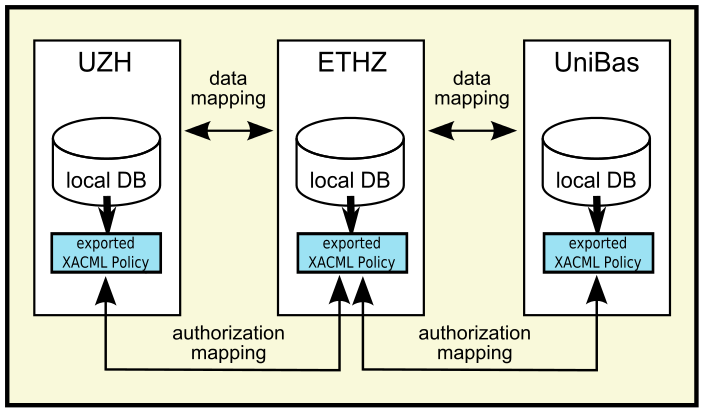
\includegraphics[scale=0.3]{demap_fig1.png}
 \end{figure}

\end{frame}

\begin{frame}[plain]{Adaptação do XACML}
\lstinputlisting[language=xml,basicstyle=\tiny,columns=fullflexible]{recursos/demap_cod1.xml}
\end{frame}

\subsubsection{Mapeamento}
  \begin{frame}{Mapeamento}
   \begin{figure}[H]
    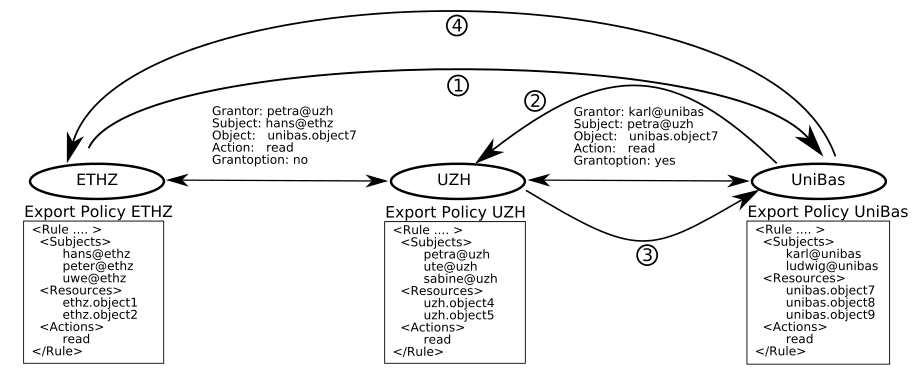
\includegraphics[scale=0.3]{demap_fig2_mp.png}
    \caption{hanz@ethz requisita unibas.object7}
   \end{figure}

  \end{frame}


\subsubsection{Diretório distribuído}
  \begin{frame}{Diretório distribuído}
   \begin{figure}[H]
    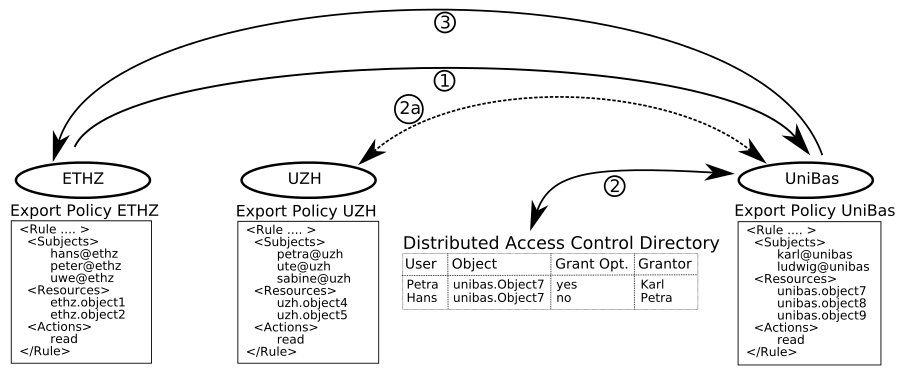
\includegraphics[scale=0.3]{demap_fig3_dd.png}
   \end{figure}

  \end{frame}
  
  \begin{frame}{Diretório distribuído - Implementação}
    \begin{itemize}
     \item Usa-se a DHT
     \item Chord
     \begin{itemize}
      \item \textit{Overhead} para manutenção do diretório
     \end{itemize}

    \end{itemize}

  \end{frame}
  
  \begin{frame}{Proteção do diretório e conteúdo distribuído}
    \begin{itemize}
     \item Cada entrada possui uma assinatura
     \item Criptografia das entradas do diretório
     \begin{itemize}
      \item Cada objeto corresponde a uma chave pública
      \item Chaves privadas são distribuídas
      \item Usa unidade certificadora centralizada
     \end{itemize}
     \item Somente o concessor pode alterar suas entradas
     \item Detecção de peers maliciosos
    \end{itemize}
   
  \end{frame}
  
  \begin{frame}{Considerações}
   \begin{itemize}
    \item Na Alteração de algum previlégio, pode ocorrer o efeito de cascata
    \item Não tem replicação
    \item Mapeamento
    \begin{itemize}
     \item Tende a criar muitas regras
     \item Mais controle
    \end{itemize}
    \item Diretório distribuído
    \begin{itemize}
     \item Política de remoção de entradas do diretório
     \item Sobrecarga da unidade certificadora
     \item Muitas entradas não serão usadas
     \item Revogação, redistribuir a chave
    \end{itemize}
   \end{itemize}
  \end{frame}


\subsection{P-Hera}
  \begin{frame}{Contexto}
   \begin{itemize}
    \item Rede não-estruturada hierárquica
    \item Primitivas: \textit{search}, \textit{get} e \textit{place}.
   \end{itemize}
   \begin{figure}[H]
      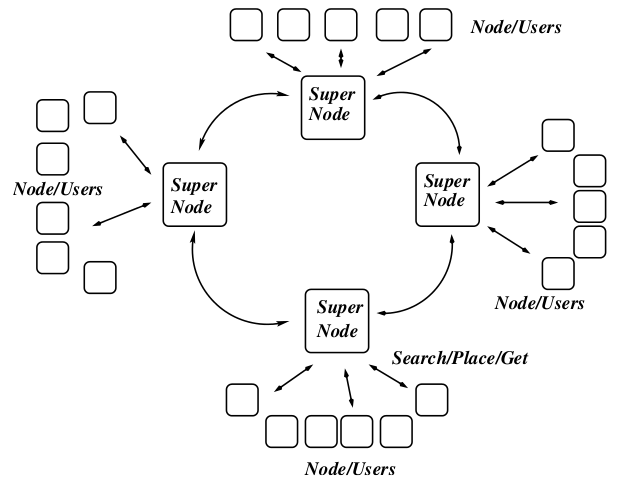
\includegraphics[scale=0.25]{phera_fig1.png}
   \end{figure}

  \end{frame}
  
  \begin{frame}{Políticas}
   \begin{itemize}
    \item Tipos:
    \begin{itemize}
     \item Política de replicação
     \item Política de armazenamento
     \item Controle de acesso
    \end{itemize}
   \end{itemize}
   \begin{figure}[H]
    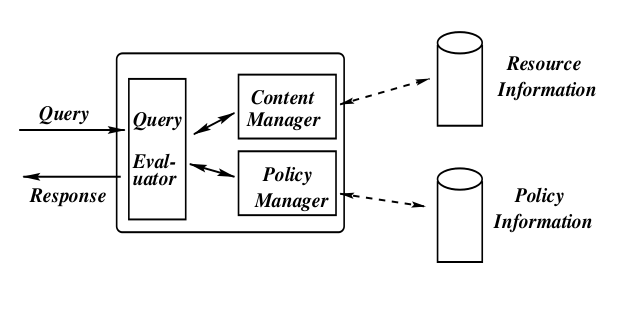
\includegraphics[scale=0.25]{phera_fig2.png}
   \end{figure}

  \end{frame}
  
  \begin{frame}{Gerenciamento de políticas}
   \begin{itemize}
    \item Armazenamento no supernodo
    \item Organização
    \begin{itemize}
     \item Sem agrupamento
     \item Agrupados por políticas
     \item Agrupados por expressões em políticas: $< attr_{i}, expr_{i} >$
    \end{itemize}

   \end{itemize}
  \end{frame}
  
  \begin{frame}{Testes}
  \begin{multicols}{2}
    \begin{figure}[H]
     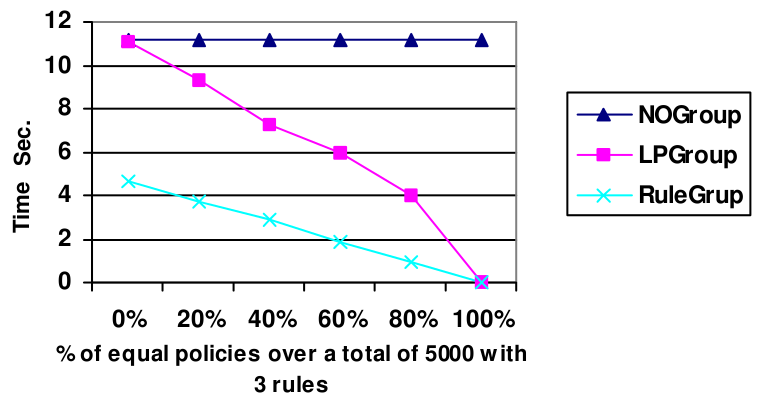
\includegraphics[scale=0.2]{phera_fig3.png}
     \caption{Avaliação de 5000 políticas}
    \end{figure}
    \begin{figure}[H]
     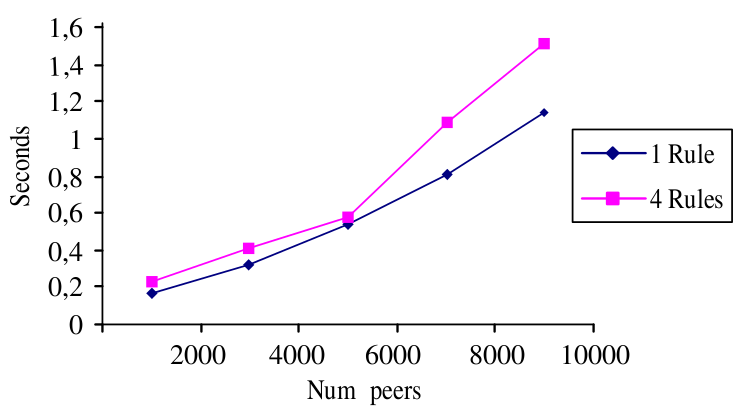
\includegraphics[scale=0.2]{phera_fig4.png}
    \end{figure}
  \end{multicols}
  \end{frame}
  
  
  \begin{frame}{Considerações}
   \begin{itemize}
    \item Preza escalabilidade
    \item Confiança em supernodos
   \end{itemize}
   

  \end{frame}






\section{Conclusão}
  \begin{frame}{Conclusão}
    \begin{itemize}
     \item Propostas para contextos específicos
     \item Tráfego extra para estabelecimento de regras
     \item Estabelecimento de confiança entre peers
    \end{itemize}

  \end{frame}


\section{Perguntas}

\begin{frame}{Perguntas}
	\begin{center}		
		\Huge PERGUNTAS?
	\end{center}
	
\end{frame}
\end{document}
